% Conceptual model for Chapter 1: awareness and capability recognition (RQ1) as
% antecedents of perceived value (RQ2, RQ3), which informs adoption intent, with
% professional field and experience as moderators.
%
% Native TikZ replacement for the former Matplotlib export fig_conceptual_model.pdf,
% whose text was outlined and therefore unsearchable and inaccessible. Flat vector,
% no gradients or drop shadows, consistent with the other figure sources here.
%
% Build:  lualatex ConceptualModel.tex  &&  cp ConceptualModel.pdf ../fig_conceptual_model.pdf
\documentclass[border=8pt]{standalone}
\usepackage{tikz}
\usetikzlibrary{positioning,arrows.meta,calc}

% Muted, print-safe fills; every box is labelled, so colour never carries meaning alone.
\definecolor{cmAwareFill}{RGB}{223,234,246}
\definecolor{cmAwareEdge}{RGB}{ 72,113,161}
\definecolor{cmValueFill}{RGB}{250,226,224}
\definecolor{cmValueEdge}{RGB}{176, 85, 78}
\definecolor{cmIntentFill}{RGB}{225,240,228}
\definecolor{cmIntentEdge}{RGB}{ 76,134, 92}
\definecolor{cmModFill}{RGB}{248,238,214}
\definecolor{cmModEdge}{RGB}{170,134, 62}
\definecolor{cmInk}{RGB}{ 34, 34, 34}
\definecolor{cmRule}{RGB}{ 90, 90, 90}

\begin{document}
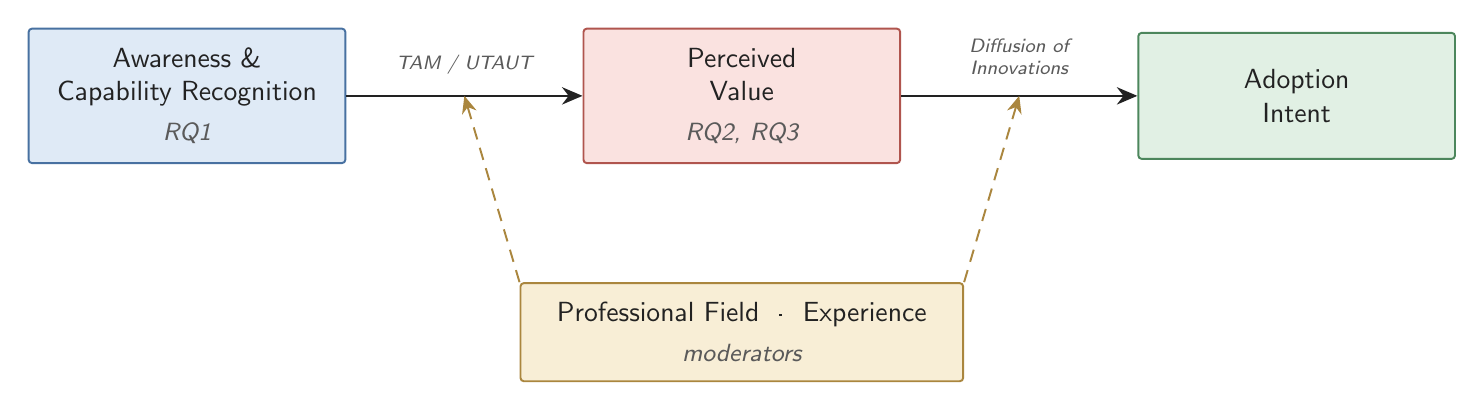
\begin{tikzpicture}[
  font=\sffamily,
  construct/.style={
    rectangle, rounded corners=1.2pt, draw, line width=0.7pt,
    text=cmInk, align=center, inner xsep=6pt, inner ysep=7pt,
    text width=36mm, minimum height=16mm,
  },
  flow/.style={-{Stealth[length=2.6mm,width=2.2mm]}, draw=cmInk, line width=0.9pt},
  moderates/.style={-{Stealth[length=2.2mm,width=1.9mm]}, draw=cmModEdge,
                    line width=0.7pt, dashed, dash pattern=on 1.6mm off 1.1mm},
  theory/.style={font=\sffamily\itshape\scriptsize, text=cmRule},
]

  % small italic grey tag used under each construct name
  \newcommand{\cmtag}[1]{{\itshape\small\textcolor{cmRule}{#1}}}

  % ---- the causal chain -------------------------------------------------
  \node[construct, fill=cmAwareFill, draw=cmAwareEdge] (aware)
    {\normalsize Awareness \&\\Capability Recognition\\[2.5pt]\cmtag{RQ1}};

  \node[construct, fill=cmValueFill, draw=cmValueEdge,
        right=30mm of aware] (value)
    {\normalsize Perceived\\Value\\[2.5pt]\cmtag{RQ2, RQ3}};

  \node[construct, fill=cmIntentFill, draw=cmIntentEdge,
        right=30mm of value] (intent)
    {\normalsize Adoption\\Intent};

  \draw[flow] (aware) -- node[theory, above=1.4mm, midway] {TAM / UTAUT} (value);
  \draw[flow] (value) -- node[theory, above=1.4mm, midway, align=center] {Diffusion of\\Innovations} (intent);

  % ---- moderators -------------------------------------------------------
  \node[construct, fill=cmModFill, draw=cmModEdge, text width=52mm,
        minimum height=12mm, below=15mm of value] (mod)
    {\normalsize Professional Field \ \textperiodcentered\ \ Experience\\[2.5pt]\cmtag{moderators}};

  \draw[moderates] (mod.north west) -- ($(aware.east)!0.5!(value.west)$);
  \draw[moderates] (mod.north east) -- ($(value.east)!0.5!(intent.west)$);

\end{tikzpicture}
\end{document}
